
\chapter{Prosody, clause types, and speech acts in English}
\label{chap:prosody}
One important source of information that we have not yet discussed is prosody. As mentioned in Section~\ref{sec:bg:theory:prosody}, the role of prosody in clause typing and speech act identification is quite complicated. This chapter focuses on English prosody and its relation with clause type and speech act. English offers an interesting case, as its interrogative clauses could be marked by morpho-syntactic features (subject-auxiliary inversion), but are also tend to be associated with a rising intonation (polar interrogative only). How should we understand the role of prosody in clause typing and speech act identification? How could the learners utilize this information in learning clause type and speech act categories? In Section~\ref{sec:prosody:bg}, I discuss the different ways people have linked English prosodic features with clause typing, and the implications for the learners. In Section~\ref{sec:prosody:children}, I review the literature on children's knowledge of prosody. Even though we do not have direct evidence for English-acquiring 18-month-olds, it is likely that they are at least sensitive to the distinction between final rise and fall. If they are indeed sensitive to this distinction, would this distinction correlate with clause types/speech acts in the input? I report results from a corpus study in Section~\ref{sec:prosody:corpus}, and use the annotated dataset to simulate whether children could learn clause types with both morpho-syntactic and prosodic information (Section~\ref{sec:prosody:model}). Results from both studies suggest that there might not be a clear correlation between final rise and clause types/speech acts, and that this prosodic feature is not informative for finding the right clause type clusters in English. I discuss the reasons for seeing these patterns in the input, and some alternative ways that prosodic information could be utilized in learning clause type clusters in Section~\ref{sec:prosody:discussion}.


\section{Background}
\label{sec:prosody:bg}
\subsection{Prosody, clause types, and speech acts in English}
In English, whether prosody is a surface feature for clause typing or simply an indicator for questioning is debated. As we have seen repeatedly, English interrogatives have their designated morpho-syntactic features, i.e. subject-auxiliary inversion. But prosodic information could also inform us about the clause type category. English declaratives tend to be associated with falling intonation, polar interrogatives tend to bear a final rising intonation, while \twh-interrogatives also generally bear a falling contour. This final rise and fall are generally believed to be the nuclear contour (\citealt{ladd1981, ladd2008intonational, hedberg2004wh, hedberg2014corpus} among many others). The nuclear contour is the contour from the nuclear pitch accent to the end of the utterance. The nuclear pitch accent is the final pitch accent (a pitch accent is a marker of greater relative prominence on a syllable). In other words, the relevant contour is the nuclear contour and whether it rises or falls. 


As we mentioned in Chapter~\ref{sec:bg:theory:prosody}, cross-linguistically languages could use morpho-syntactic features alone, prosodic alone, or a combination of both for clause typing. We also tentatively put English in the ``combination'' column. But is the final rise a property of English interrogatives? Or is it simply a property of questionhood, and that some interrogatives are associated with this feature because they are used to perform questioning acts? To address this issue, we should look at the cases where speech acts and clause types misalign. Specifically, when imperatives and declaratives and imperatives are used to ask questions, and when interrogatives are used to perform assertions and requests.

In Chapter~\ref{sec:engcl:bg:grammar}, I argued that rising declaratives are declaratives that can be used to ask questions. But declarative questions do not need to be associated with final rise. Embedded questions like (\ref{ex:prosody:embedq}) are declaratives used to perform questions, but the most natural prosodic contour associated with it should be the same as declarative assertions.

\bex{ex:prosody:embedq}
I wonder if you could tell me what time it is.
\eex

Similarly, imperatives used to perform questions like (\ref{ex:prosody:impq}) could also have falling intonation:

\bex{ex:prosody:impq}
Tell me what time it is.
\eex

When used to perform assertive acts, both polar and \twh-interrogatives tend to be associated with a final fall. The following example comes from a production study by \textcite{dehe2020rhetoric}:
\bex{ex:prosody:dehe}
Context: One of your friends suggest that you should all go to the museum. But it is known to all of your friends that none of your friends likes to go to the museum, and therefore nobody responded to his suggestion. You say to your friend: 
\eex
\begin{figure}[H]
\begin{center}
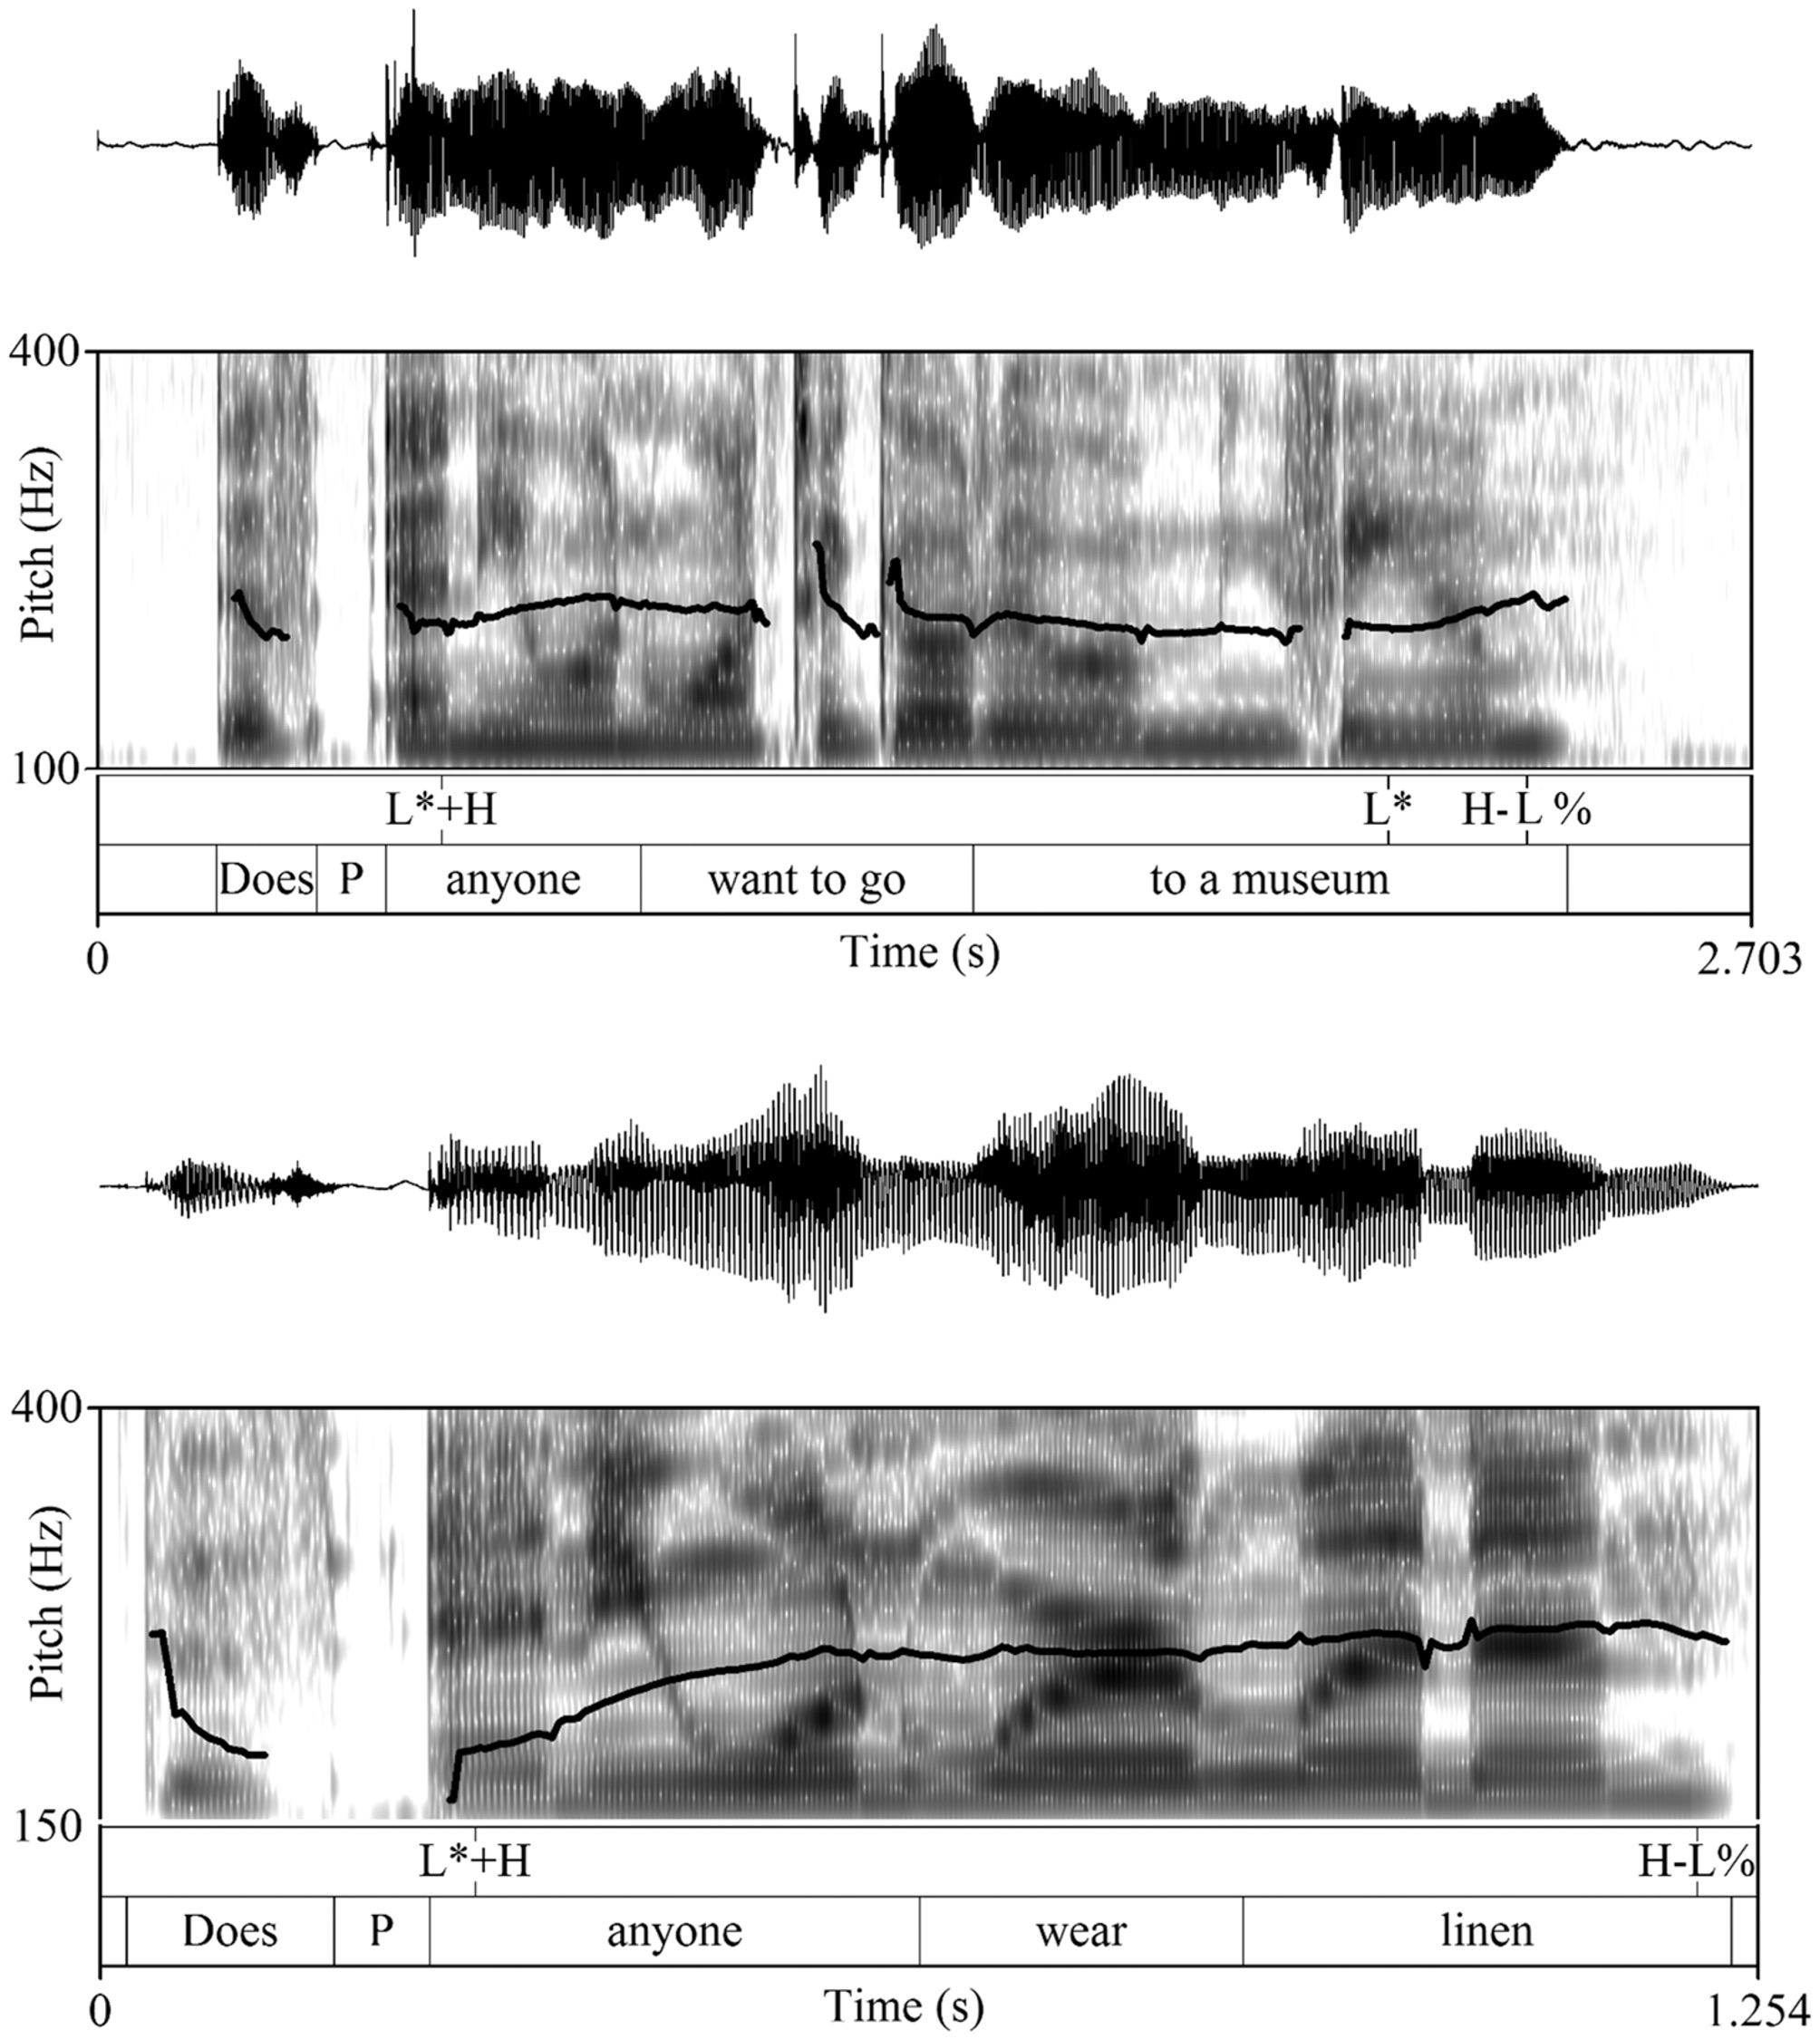
\includegraphics[width = 0.7\textwidth]{figures/rhe-polar.jpg}
	\caption{Two types of frequent rhetorical polar interrogatives produced by a female (up) and male (down) participant with contexts similar to (\ref{ex:prosody:dehe}) (Figure~11 from \cite{dehe2020rhetoric}) }\label{fig:rhe-polar}
\end{center}
\end{figure}

But \textcite{dehe2020rhetoric} also note that a substantial amount of sentences are produced with final rise H-H\% (examples are not given in the paper). 

When interrogatives are used to perform requests like \tit{Can you pass the salt?} the most natural prosodic contour seems to be the regular polar interrogative contour. 

To summarize, declaratives and imperatives used to ask questions have final rises (rising declaratives), but also have falling intonation (embedded questions). Interrogatives used to perform an assertion  or a request are associated with a rising intonation. These patterns seem to suggest that English final rise (a rising nuclear contour) could be triggered by a question act, but could also be triggered by the right matrix clause type (polar interrogatives).  


%In addition to these misaligned cases, there are some other cases that suggest that final rise %fragments



\subsection{Children's knowledge of prosodic features}
\label{sec:prosody:children}
As we have seen in Chapter~\ref{chap:background}, rising intonation tends to associate with interrogatives (particularly polar interrogatives) and questions cross-linguistically. Results from previous experimental and corpus studies suggest that children might be sensitive to the distinction between a final rise (specifically polar interrogative rise) and a final fall. 

From as early as 6 months old, infants are able to identify utterance boundaries, and are sensitive to the edge prosody (\cite{johnson2014edge}). They also can use distinctions in prosodic contours (e.g. final rise vs. fall) to distinguish clause types (polar interrogative vs. declaratives). For example, \textcite{frota2014}) show that as young as 6 months old, European Portuguese-acquiring infants are sensitive to the prosodic distinction between polar interrogatives and declaratives, where prosody is the only cue that distinguishes these two clause types in the language. \textcite{geffenmintz2011} find that when given a combination of word order and prosodic cues, English-acquiring 7-month-olds can distinguish polar interrogatives from declarative assertions. \textcite{soderstrom2005clause} test English-speaking infants between 4.5 months and 2 years old (average 14 months old), and find that they are sensitive to the distinction between declaratives with a falling a rising contour. Before 18 months old, infants acquiring non-lexical tone languages such as English are shown to be sensitive to some tonal distinctions in lexical tone languages such as Mandarin. They are particularly sensitive to the distinction between the rising tone that is similar to English polar-interrogative rise, and the falling tone similar to English declarative fall (\cite{shi2017tone, Hay2019}), although it is unclear whether we can draw any conclusions about their sensitivity to English polar interrogative rise.

While infants might be sensitive to the distinction between rise and fall, it is unclear, at least for English-acquiring infants, whether they can use prosodic cues alone to detect questions. When given only prosodic cues without any morpho-syntactic information, \textcite{keitel2013turn} and \textcite{casillas2017turn} both find that children younger than 2 years old cannot use intonation alone to infer transition after a turn (i.e. casting more anticipatory looks to the addressee), but they can infer such transitions with morpho-syntactic cues associated with interrogatives. However, the low-pass filtered utterances might be difficult for infants to process, so their failure at casting anticipatory looks after rising intonation might be an artifact of task effect.

On the production side, studies have found that children are able to use different prosodic contours for different functions from when they start speaking. \textcite{menyuk1969prosody} analyze the prosodic contours of one child's utterances, and annotates their perceived speech acts between 18  and 20 months, and find that even though the utterances are mostly one word or two words, there's a correlation between the intended speech act and prosody. For example, an intended request with a one-word utterance ``door!'' is typically associated with a sharp rise and then fall; the same utterance as a question tends to end with a rising intonation. Since the speech act labels in the study are annotations by adults inferred from one-word utterances, it is unclear whether these are actually the speech acts that the child perform, and the conclusion seems to be that adults systematically associate certain prosodic contours to \aqrs{}, even with one-word utterance. Nonetheless, it seems that at the child is using different prosodic contours at this age, and it is possible that these contours are systematically associated with different speech acts. 

Furthermore, for their own production, children seem to associate the rising contour with response elicitation. \textcite{flax1991prosody} conduct a longitudinal study observing three children interacting with their mothers before they can speak (when they have a vocabulary of 10 words, and again when their vocabulary consists of 50 words), and code whether the child's utterance (or vocalization, at the pre-verbal stage) is produced with a final rise. They find when children request a response from their addressee, they tend to produce the utterance with a final rise. 

Previous studies have also shown that there are prosodic cues that distinguish clause types and speech acts, in particular to distinguish polar interrogatives and declaratives, in child-directed speech. \textcite{geffenmintz2017final} show that polar interrogatives and declaratives differ in the pitch of the last two syllables, with polar interrogatives generally have a rising contour; they also find that there is no distinction between \twh-interrogatives and declaratives in the last two syllables. \textcite{chianggeffenmintz2018initial} examine sentence-initial prosodic cues, and find that polar interrogatives and declaratives both have a higher starting pitch than declaratives, and that echo \twh-questions tend to have a higher pitch than other types of questions. %These studies only looked at the duration, F0, and intensity of the last two and the first syllables; there might be 

In sum, prosodic cues are in principle helpful for distinguishing different speech acts, and there is evidence suggesting that children can perceive these cues. In particular, there might be cues at sentence-final and sentence-initial position that are both useful and available to children. We do not have sufficient data to know whether 18-month-olds are sensitive to the prosodic distinctions between declaratives and polar interrogatives, but evidence from other languages suggests that infants around this age are at least sensitive to the final fall vs. rise distinction. If children are indeed sensitive to this distinction, would they find anything in the input? In the next section, I report results from a corpus study examining the prosodic features of parents' speech acts and clause types.

\section{Corpus study}
\label{sec:prosody:corpus}


\subsection{Methods}
\label{sec:engsp:corpus:method}
This study also used data from the Providence Corpus (\citealt{ProvidenceCorpus}) from CHILDES system (\citealt{CHILDES}). The audio and video of the sessions sampled in Chapter~\ref{chap:eng-cl} were extracted for annotation. 

For the audio data, I adapted a Kaldi forced alignment system (\cite{kaldi}) to obtain a time-aligned dataset containing the beginning and ending timestamp of each utterance in a session. I also manually aligned 20\% of this dataset to compare for accuracy. The mean difference between the manually aligned dataset and the forced-aligned dataset is 0.1s at the beginning of the utterance (0.001s to 20s), and 0.08s at the end of the utterance. We then extracted the pitch information of each utterance using a Python library for the Praat software (\cite{praat}), Parselmouth (\cite{parselmouth}). 


The pitch information from 3366 utterances were extracted by using Praat (\citealt{praat}). I further applied a low-pass filter at 500 Hz that removes most of the phonetic information used to distinguish between phonemes. 

As discussed in the previous section, what we are most interested in is the nuclear contours and whether they rise or fall. The nuclear contour is defined as the contour from the nuclear pitch accent to the end of the utterance; the nuclear pitch accent is the final pitch accent, and a pitch accent is just a marker of greater relative prominence on a syllable (\cite{buring2016intonation}). To my knowledge, there is currently no perfect way to automate recognition of (nuclear) pitch accents (see \cite{buring2016intonation} for a discussion). I therefore applied the following algorithm to identify the nuclear contours of these 3366 utterances, and hand-annotated 100 for comparison. I first applied a peak identification algorithm (\textsf{scipy.signal.find\_peaks}; from the scipy python package). This function takes a 1-D array and finds all local maxima by simple comparison of neighboring values. The peaks in F0 would be our approximation for the pitch accent (most prominent syllable). But prominence is a perceptual category: a syllable that is prominent is in some sense intuitively "stronger" than surrounding syllables, according to human intuition. This could either be the highest or lowest F0. I therefore inverted the pitch track and applied the find peak algorithm again; the results would be a set of valleys in the pitch track. The last peak or valley was then considered the last pitch accent. If this last ``pitch accent'' is a peak like (\ref{fig:rise-example}), then the utterance was labelled as having a final rising contour.\footnote{The script for coding pitch information can be found at \mycode{}.} If the last ``pitch accent'' is a valley, then the ``nuclear contour'' was considered a rise. 

 
\begin{figure}[H]
    \centering
    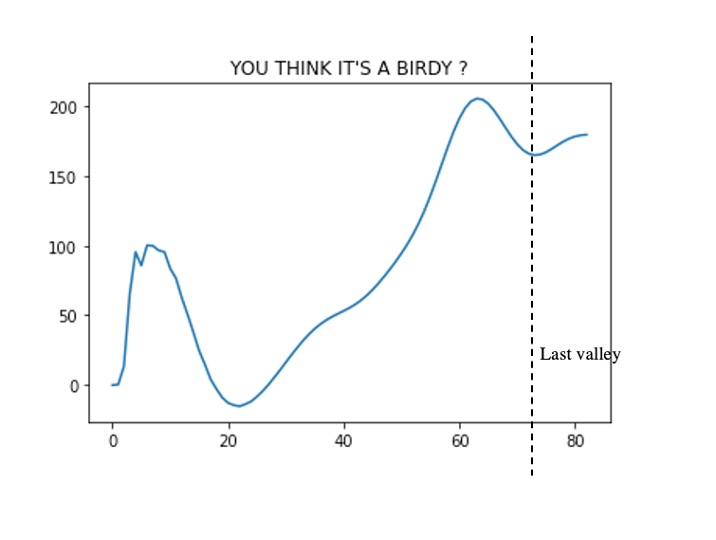
\includegraphics[width=0.7\textwidth]{figures/pitch-rise.jpg}
    \caption{``You think it's a birdy?''}
    \label{fig:rise-example}
\end{figure}


I then manually annotated 100 utterances to check for accuracy; 52 of these were correctly labeled by the algorithm. The low agreement rate could be due to a number of factors. Besides the fact that the recordings themselves are noisy, one of the problems with automating the process is that the tail end of all pitch tracks can be distorted in some way. The reason is that pitch periods are irregular due to dissipating energy, which may cause spurious events in the waveform to be misinterpreted as a pitch period, which Praat then incorrectly interprets as pitch. I plan to hand annotate more utterances, and improve the algorithm.


%Finally, you give the plots you already have in this subsection, and you say, despite being a noisy approximation of the actual data, you found some signal where it matters (polar interrogatives have more rises!). And so the child might be using this, and you say that you plan to look at higher quality hand annotated data in future work. (You don't need to put this in, but I think you might also hope to improve the automated categorization as well.)


For prosodic patterns, we should see that final rising contour is more frequently associated with questions, especially polar interrogatives, than with assertions.

\subsection{Results}
\label{sec:engsp:results:prosody}

Figure~\ref{fig:rise-sp} and \ref{fig:rise-cl} show the proportion of final rise, as identified by the algorithm. As we can see, there is no difference in the proportion of rises among speech acts. 

\begin{figure}[H]
    \centering
    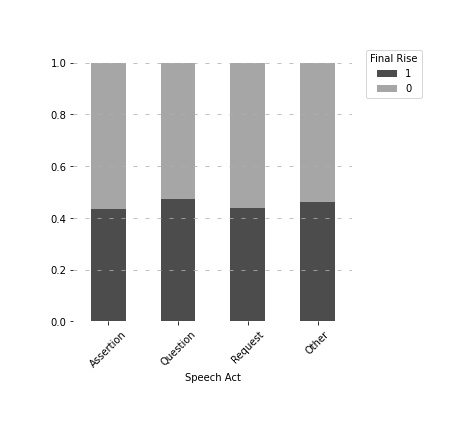
\includegraphics[width=0.7\textwidth]{figures/rise-sp.jpg}
    \caption{Proportion of utterances with final rise across different speech acts}
    \label{fig:rise-sp}
\end{figure}


\begin{figure}[H]
    \centering
    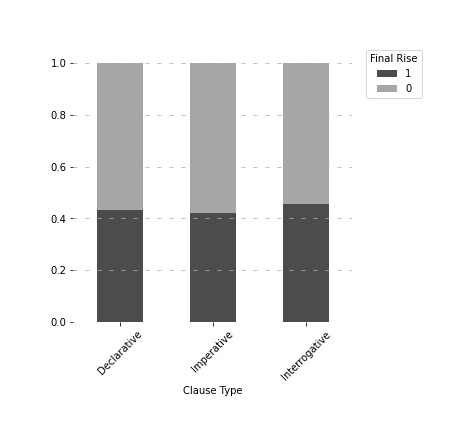
\includegraphics[width=0.7\textwidth]{figures/rise-cl.jpg}
    \caption{Proportion of utterances with final rise across different clause types}
    \label{fig:rise-cl}
\end{figure}

But if we look into sub-categories of interrogatives, we can see that the proportion of final rise is much higher with polar interrogatives than with declaratives. 
\begin{figure}[H]
    \centering
    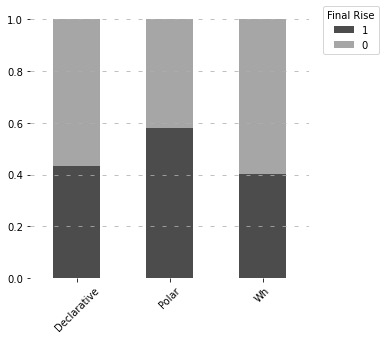
\includegraphics[width=0.7\textwidth]{figures/pitch-polardecwh.jpg}
    \caption{Proportion of declaratives, \twh{} and polar interrogatives with final rise}
    \label{fig:rise-int}
\end{figure}

Despite being a noisy approximation of the actual data, I found that some signal for polar interrogatives, as predicted. Specifically, polar interrogatives are more often associated with final rises than declaratives and \twh-interrogatives.

These results also seem to suggest that the presence of final rise might not be informative of the speech act of the sentence, unless morpho-syntactic features like subject-auxiliary inversion is also present. However, this could be a result of the algorithm I applied here, and do not reflect the pattern of the data. I plan to hand annotate more cases in the future to have more reliable data.

\section{Learning clause type categories with prosody}\label{sec:prosody:model}

Our next question is, would prosodic information help the two learners (\distlearner{} and \praglearner{}) find the right clause type clusterings. If prosody helps, then the performance of \dlearnerabbr{} will improve with the addition of prosodic information, and the model should be able to find the right clusterings. To this end, I modified the models given in Chapter~\ref{chap:eng-cl} to include prosodic information. The modified models are given below:


%As discussed in the previous sections, whether prosody is informative for both clause types and speech acts or speech act alone in English is an open issue. I also discussed in Chapter~\ref{sec:bg:theory:prosody} that there are languages that do not utilize intonation in clause typing. We can either assume that children have an innate knowledge that prosody informs clause typing, and hope the input might be such that prosody is uninformative; or we can assume that children only know \tit{a priori} prosody informs speech act categorization, and not clause type categorization. Since at this point, we are assuming that the speech act information is either inaccessible to the learner (the \dlearnerabbr{} model) or is known to the learner (the \plearnerabbr{} model), if prosody is only informative to speech act and not clause type, this source of information would be redundant for the models. Therefore, we are adopting the assumption that prosody informs clause typing.

\begin{figure}[H]
\begin{minipage}[b]{0.45\linewidth}
\begin{center}
\begin{tikzpicture}
\node[latent] (c) {$C_{i}$};
\node[obs, below=of c, xshift=-0.6cm] (s) {$\vec{S_{i}}$};
\node[obs, below=of c, xshift=0.6cm] (i) {$I_{i}$};
\node[latent, right=of i] (lambda) {$\lambda^{c}$};
%\node[const, right=of lambda] (eta) {$\eta$};
\node[latent, right=of c] (phi) {$\phi$};
%\node[const, right=of phi] (beta) {$\beta$};
\node[latent, left=of s] (delta) {$\delta^{(c)}$};
%\node[const, left=of delta] (gamma) {$\gamma$};


\edge {phi}{c};
\edge {c}{s};
\edge {delta}{s};
%\edge {beta}{phi};
%\edge {gamma}{delta};
\edge {lambda, c}{i};
%\edge {eta}{lambda};


\plate {nutt}{(c)(s)(i)}{$N$};
\plate {cvalue}{(delta)}{$C$};
\plate {fvalue}{(cvalue)(s)}{$F$};
%\plate {fvalue}{(gamma)(delta)(s)(cvalue)}{$F$};
\end{tikzpicture}
\end{center}
%\caption{Hierarchical model with all parameters specified}\label{fg:model}
\end{minipage}
\hspace{0.6cm}
\begin{minipage}[b]{0.45\linewidth}
\begin{center}
\begin{tikzpicture}
\node[obs] (a) {$A_{i}$};
\node[latent, right=of a] (theta) {$\theta$};
%\node[const, right=of theta] (alpha) {$\alpha$};
\node[latent, below=of a] (c) {$C_{i}$};
\node[obs, below=of c, xshift=-0.6cm] (s) {$\vec{S_{i}}$};
\node[obs, below=of c, xshift=0.6cm] (l) {$I_{i}$};
\node[latent, right=of l] (lambda) {$\lambda^{c}$};
%\node[const, right=of lambda] (eta) {$\eta$};
\node[latent, right=of c] (phi) {$\phi^{(a)}$};
%\node[const, right=of phi] (beta) {$\beta$};
\node[latent, left=of s] (delta) {$\delta^{(c)}$};
%\node[const, left=of delta] (gamma) {$\gamma$};

\edge {theta}{a};
%\edge {alpha}{theta};
\edge {phi, a}{c};
\edge {delta, c}{s};
%\edge {beta}{phi};
%\edge {gamma}{delta};
\edge {c,lambda}{l};
%\edge {eta}{lambda};


\plate {nutt}{(a)(c)(s)(l)}{$N$};
\plate {avalue}{(phi)}{$A$};
\plate {cvalue}{(delta)}{$C$};
\plate {fvalue}{(delta)(s)(cvalue)}{$F$};
\end{tikzpicture}
\end{center}
\end{minipage}
\caption{The \distlearner{} model with prosody (left) and \praglearner{} model with prosody (right)}\label{fig:prosody:model}
\end{figure}


Both model now learns from prosodic data, represented in Figure~\ref{fig:prosody:model} as $I_{i}$. This variable is a Bernoulli variable conditioned on $c_{i}$. It takes the value 1 if the sentence is associated with a final rise intonation, and 0 otherwise. It is also conditioned on the parameter $\lambda^{(c)}$, which represents the probability of observing a final rise in a particular clause type category. 

The same sampling method as reported in Chapter~\ref{sec:engcl:model} was used. The posterior of $c_{i}$ is updated with the following equations:


\begin{equation}\label{CfromSI}
\begin{split}
p(c_{i}| c_{-i}, \vec{a}, \beta, \vec{S_{i}}, \delta, \gamma, l_{i}, \lambda, \eta) = &
\frac{p(\vec{S_{i}}| \vec{c}, \delta, \gamma)\ p(l_{i} |\vec{c},\lambda, \eta)\ p(c_{i}|\beta, c_{-i})}{\Sigma_{c_{i}'}p(\vec{S_{i}}| \vec{c'}, \delta, \gamma)\ p(l_{i} |\vec{c'},\lambda, \eta)\ p(c_{i}'|\beta, c_{-i})}\\
=& \frac{ \prod_{F}\frac{\gamma_{0}+n_{s^{F, c_{i}}_{i}}}{2r_{0}+n_{c^{F}_{i}}}%S
\frac{\eta_{0}+n_{l_{i}}^{c_{i}}}{2\eta_{0}+n_{c_{i}}}%L
\frac{\beta_{0}+n_{c_{i}}}{3\beta_{0}+n}%C
}%分子
{\sum_{c'_{i}}\prod_{F}\frac{\gamma_{0}+n^{F, c'_{i}}_{s_{i}}}{2r_{0}+n^{F}_{c'_{i}}}%S
\frac{\eta_{0}+n_{l_{i}}^{c'_{i}}}{2\eta_{0}+n_{c'_{i}}}%L
\frac{\beta_{0}+n_{c'_{i}}}{3\beta_{0}+n} %C
}%分母
\end{split}
\end{equation}

\begin{equation}\label{CfromSIA}
\begin{split}
p(c_{i}| c_{-i}, \vec{a}, \beta, \vec{S_{i}}, \delta, \gamma, l_{i}, \lambda, \eta) = &
\frac{p(\vec{S_{i}}| \vec{c}, \delta, \gamma)\ p(l_{i} |\vec{c},\lambda, \eta)\ p(c_{i}|\beta, c_{-i}, \vec{a})}{\Sigma_{c_{i}'}p(\vec{S_{i}}| \vec{c'}, \delta, \gamma)\ p(l_{i} |\vec{c'},\lambda, \eta)\ p(c_{i}'|\beta, c_{-i}, \vec{a})}\\
=& \frac{ \prod_{F}\frac{\gamma_{0}+n_{s^{F, c_{i}}_{i}}}{2r_{0}+n_{c^{F}_{i}}}%S
\frac{\eta_{0}+n_{l_{i}}^{c_{i}}}{2\eta_{0}+n_{c_{i}}}%L
\frac{\beta_{0}+n_{c_{i}}^{a_{i}}}{4\beta_{0}+n_{a_{i}}}%C
}%分子
{\sum_{c'_{i}}\prod_{F}\frac{\gamma_{0}+n^{F, c'_{i}}_{s_{i}}}{2r_{0}+n^{F}_{c'_{i}}}%S
\frac{\eta_{0}+n_{l_{i}}^{c'_{i}}}{2\eta_{0}+n_{c'_{i}}}%L
\frac{\beta_{0}+n_{c'_{i}}^{a_{i}}}{4\beta_{0}+n_{a_{i}}} %C
}%分母
\end{split}
\end{equation}

The data for this model were taken from the annotated dataset reported in the last section. In total, $3366$  sentences were fed into the models.


Overall, these two models do not improve on the models without prosody, as shown by the similar adjusted rand score in Figure~\ref{fig:prosody:compare}.

\begin{figure}[H]
    \centering
    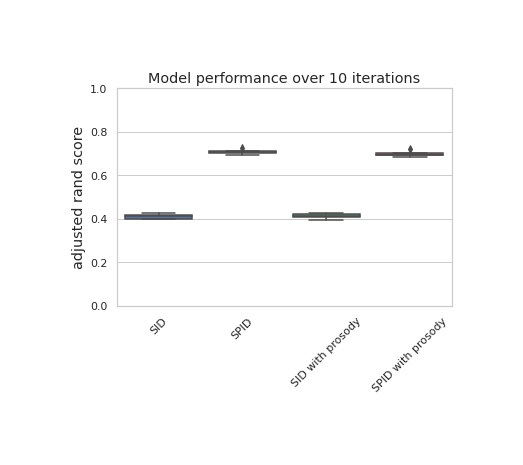
\includegraphics[width=0.8\textwidth]{figures/compare-adjusted-bu.jpg}
    \caption{Performance of all four models as measured by adjusted rand score }
    \label{fig:prosody:compare}
\end{figure}

The clusters identified by the two models with prosody also do not improve on previous models. As shown by Figure~\ref{fig:heatmap-prosody} and Figure~\ref{fig:heatrev-prosody}, \dlearnerabbr{} with prosody still cannot identify the right clusters, and \plearnerabbr{} could find the right clusters. 
\begin{figure}[H]
\begin{minipage}[b]{0.45\linewidth}	
    \centering
    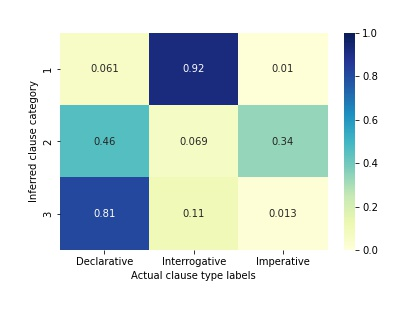
\includegraphics[width=1.2\textwidth]{figures/baseline-heatmap-bu.jpg}
\end{minipage}
\begin{minipage}[b]{0.45\linewidth}	
\centering
    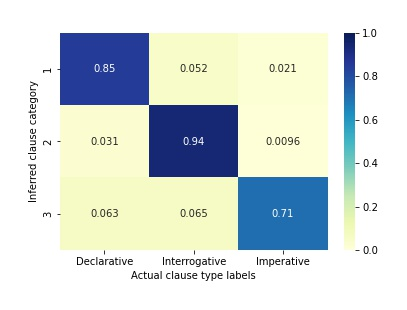
\includegraphics[width=1.2\textwidth]{figures/target-heatmap-bu.jpg}
\end{minipage}
    \caption{The proportion of \diis{} in each of the three clusters identified by the \dlearnerabbr{} with prosody (left) and the \plearnerabbr{} model with prosody (right). }
    \label{fig:heatmap-prosody}
\end{figure}

\begin{figure}[H]
\begin{minipage}[b]{0.45\linewidth}	
    \centering
    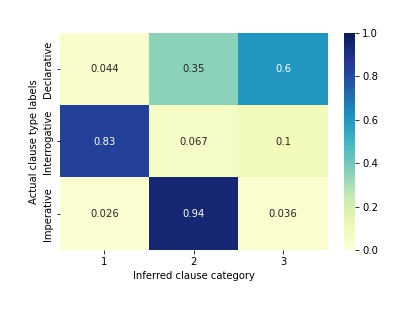
\includegraphics[width=1.2\textwidth]{figures/baseline-heatrev-bu.jpg}
\end{minipage}
\begin{minipage}[b]{0.45\linewidth}	
    \centering
    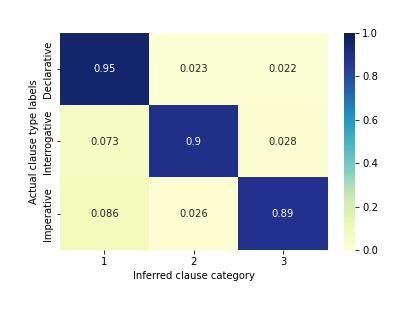
\includegraphics[width=1.2\textwidth]{figures/target-heatrev-bu.jpg}
\end{minipage}   
    \caption{The proportion of actual \diis{} clustered in one category as identified by the \dlearnerabbr{}+prosody model (right) and \plearnerabbr{}+prosody model (left) }
    \label{fig:heatrev-prosody}
\end{figure}

Figure~\ref{fig:baseline-syncluster-prosody} and Figure~\ref{fig:target-syncluster-prosody} show the surface features identified by the two models with prosody. Again, the \dlearnerabbr{} with prosody cannot identify [$-$ subject] for imperatives, and \plearnerabbr{} can.  



\begin{figure}[H]
    \centering
    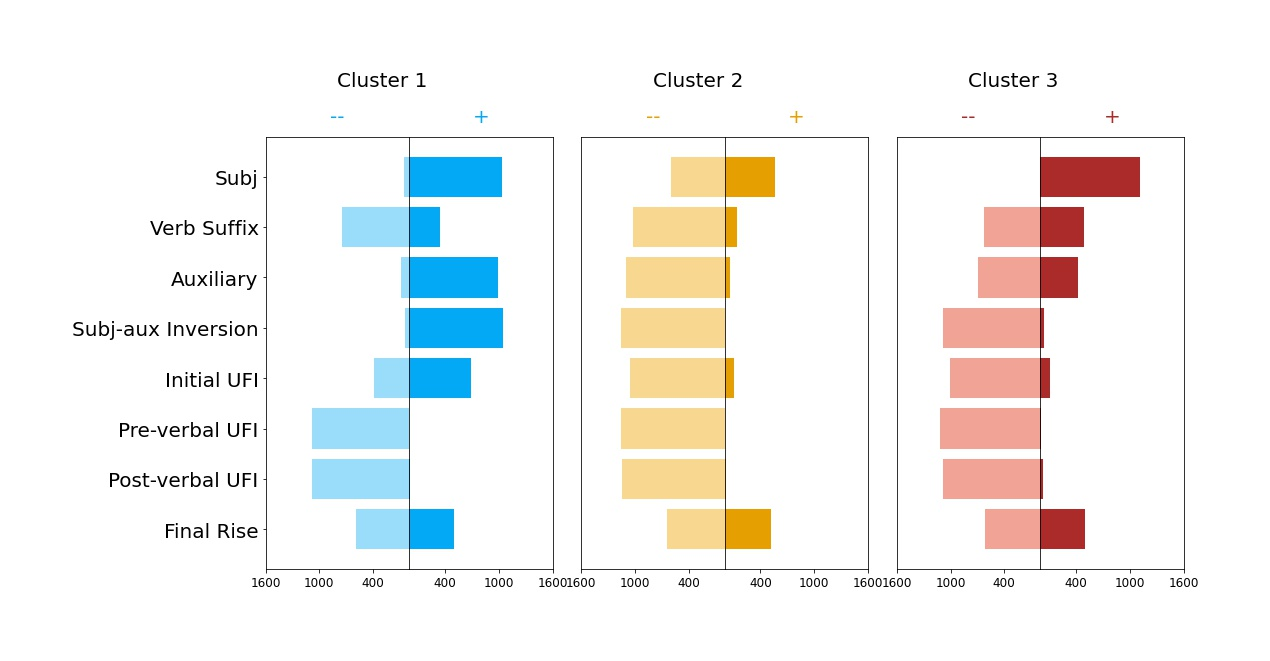
\includegraphics[width=1\textwidth]{figures/baseline-syncluster-bu.jpg}
    \caption{\revise{The morpho-syntactic profile of each cluster identified by the \dlearnerabbr{}+prosody model (Cluster 1 $\sim$Interrogatives , Cluster 2 $\sim$ Imperatives, Cluster 3 $\sim$ Declaratives).}}
    \label{fig:baseline-syncluster-prosody}
\end{figure}

\begin{figure}[H]
    \centering
    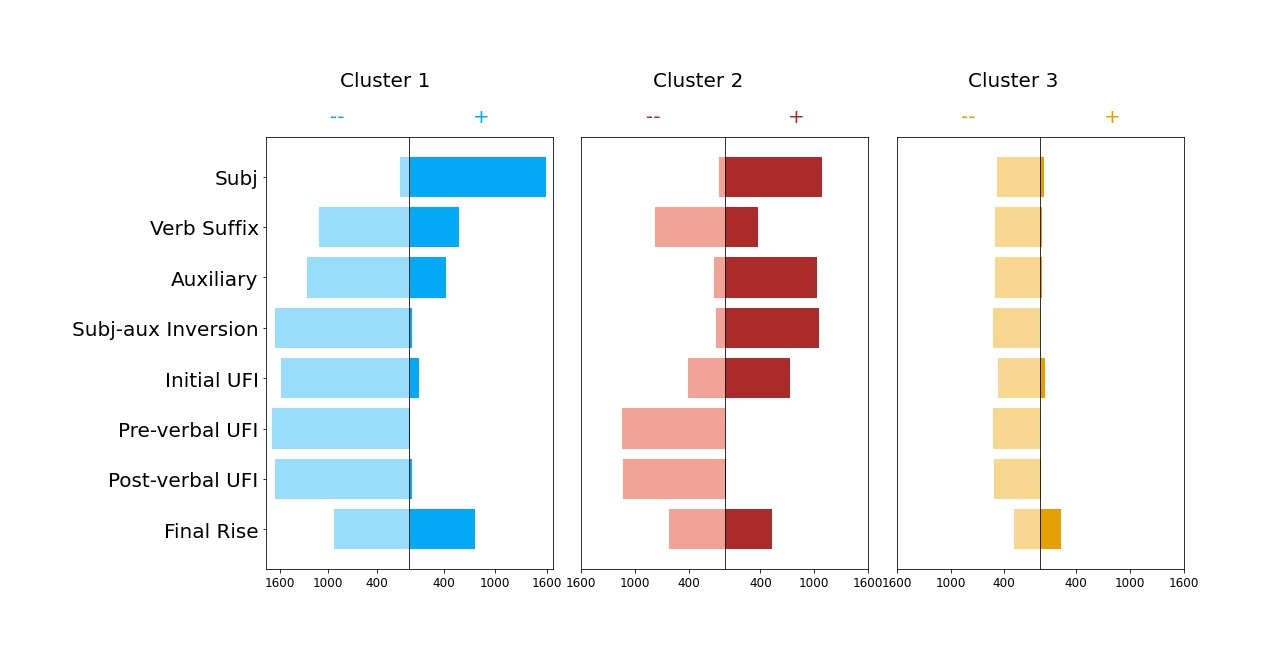
\includegraphics[width=1\textwidth]{figures/target-syncluster-bu.jpg}
    \caption{\revise{The morpho-syntactic profile of each cluster identified by the \plearnerabbr{}+prosody model (Cluster 1 $\sim$ Declaratives , Cluster 2 $\sim$ Interrogatives, Cluster 3 $\sim$ Imperatives ).}}
    \label{fig:target-syncluster-prosody}
\end{figure}

Results from our simulations suggest that prosodic features do not improve the performance of \dlearnerabbr{}; pragmatics is still necessary for finding the right clusters.


\section{Discussion}
\label{sec:prosody:discussion}
Cross-linguistically, pitch rises tend to signal questions and pitch falls signal assertions; and some argue that this universality reflects the innate knowledge that high pitch connects to the speech act of questioning (\cite{ohala1984,gussenhovenchen2000,gussenhoven2002} among others). If children are armed with the knowledge that questions tend to be associated with rising contours, they might expect rising contours to be somewhat correlated with the act of asking a question. But just as not all interrogatives have subject-auxiliary inversion, not all questions have final rises. With preliminary data, I found that parents do not use final rises more often with questions, but polar interrogatives have more final rises than other types of speech acts and clause types, including \twh-interrogatives and declaratives. Adding prosody to the \dlearnerabbr{} and \plearnerabbr{} models does not improve their performances. 


The correlation between final rise is not with the questioning speech act, but with a specific type of interrogative. Since our model assumes that the presence of final rise predicts the use of declaratives and interrogatives as a whole, this additional information did not improve the models' performances. However, it is possible that the contribution of prosody is more complicated. For example, the learner might need to combine prosody with some morpho-syntactic features for this information to be useful. Learners might first come to associate polar interrogatives with questions. They might they be able to bootstrap other interrogatives to questions by noticing similarities in morphosyntax (e.g.,~whether there is subject-auxiliary inversion). %Thus, a bootstrapping strategy relying on prosody to figure out clause typing would have to be incremental: learners would first come to associate a subset of interrogatives to questions, and then would have to rely on additional correlations in morpho-synatctic and/or pragmatic features to figure out the other interrogatives.

It is also possible that instead of three categories, the models perform better identifying four categories, with polar and \twh-interrogatives separated. These two types of interrogatives share the same sentential force, but not the same set of morpho-syntactic or prosodic features. Polar interrogtives do not have \twh-phrases and are associated with final rises, but \twh-interrogatives have \twh-phrases and are associated with final falls. It is then likely that they should not be treated as a unified category by the learner. I leave these explorations to future research. 

%%%%%%%%TRYTHIS
%